\documentclass{article}
\usepackage[utf8]{inputenc}
\usepackage{amsmath, amssymb, tikz, graphicx}
\usepackage{multicol}
\usepackage{enumitem}
\usepackage{graphicx}
\usepackage[margin=1in]{geometry} % Paquete geometry para ajustar márgenes
\usepackage{float}
\usepackage{hyperref}
\usepackage{pgfplots}
\usepackage{listings}
\usepackage{xcolor}

\usepackage{parskip} % Ajusta el espacio entre párrafos

\setlength{\parindent}{1.5em} % Ajusta la longitud de la sangría
\setlength{\parskip}{0.5em} % Ajusta el espacio entre párrafos

\pgfplotsset{compat=1.18}

% Definir el estilo "jupyter" para el código  
\lstdefinestyle{jupyter}{  
    backgroundcolor=\color{gray!10},  
    basicstyle=\ttfamily\small,  
    keywordstyle=\color{blue},  
    commentstyle=\color{green!60!black},  
    stringstyle=\color{red},  
    breaklines=true,  
    frame=single,  
    language=Python,
    extendedchars=true,
    inputencoding=utf8,
    showspaces=false,        % Desactiva la visualización de espacios
    showstringspaces=false   % Desactiva la visualización de espacios en cadenas
}  

% Definiendo los caracteres especiales
\lstset{
  inputencoding=utf8/latin1,
  extendedchars=true,
  literate={á}{{\'a}}1 {é}{{\'e}}1 {í}{{\'i}}1 {ó}{{\'o}}1 {ú}{{\'u}}1
           {Á}{{\'A}}1 {É}{{\'E}}1 {Í}{{\'I}}1 {Ó}{{\'O}}1 {Ú}{{\'U}}1
           {ñ}{{\~n}}1 {Ñ}{{\~N}}1 {¿}{{¿}}1 {¡}{{¡}}1 {≈}{{$\approx$}}1
           {≤}{{$\leq$}}1 {≥}{{$\geq$}}1 {≠}{{$\neq$}}1 {√}{{$\sqrt{}$}}1
           {∞}{{$\infty$}}1 {α}{{$\alpha$}}1 {β}{{$\beta$}}1 {γ}{{$\gamma$}}1
           {δ}{{$\delta$}}1 {ε}{{$\varepsilon$}}1 {θ}{{$\theta$}}1 {λ}{{$\lambda$}}1
           {μ}{{$\mu$}}1 {π}{{$\pi$}}1 {ρ}{{$\rho$}}1 {σ}{{$\sigma$}}1
           {τ}{{$\tau$}}1 {φ}{{$\phi$}}1 {ω}{{$\omega$}}1
           {Γ}{{$\Gamma$}}1 {Δ}{{$\Delta$}}1 {Θ}{{$\Theta$}}1 {Λ}{{$\Lambda$}}1
           {Π}{{$\Pi$}}1 {Σ}{{$\Sigma$}}1 {Φ}{{$\Phi$}}1 {Ω}{{$\Omega$}}1
}


\title{Cálculo Integral I-2025 301-302}
\author{Johan Sebastián Posada Beltrán}
\date{\today}

\begin{document}

\maketitle

\section{Repositorio}

En el siguiente enlace se encuentra el repositorio de GitHub con el código \LaTeX y Python que se usó para realizar la tarea: \url{https://github.com/johanP051/tareaII-calculoII/tree/main/latex}
\section{Repaso}

\begin{enumerate}
    \item Defina la integral definida y explique su interpretacion geométrica
\end{enumerate}

La integral definida se define como:
\[
\int_{a}^{b} f(x) \,dx = \lim_{n \to \infty} \sum_{i=1}^{n} f(x_i^*) \Delta x
\]
Donde $f(x)$ es continua en el intervalo \([a,b]\), que se divide en \(n\) subintervalos de igual longitud \(\Delta x\), y \(x_i^*\) es el punto medio entre \(x_{i-1}\) y \(x_i\).
La integral significa el área bajo la curva de la función \(f(x)\) en el intervalo \([a,b]\). Cuando n tiende a infinito, la suma de Riemann se convierte en el área exacta bajo la curva, ya que los rectángulos se hacen más pequeños y se ajustan mejor a la gráfica de la función.

\begin{enumerate}
    \setcounter{enumi}{1}
    \item Calcule la suma de Riemann izquierda para \( f(x) = x^2 \) en \([0,1]\) con \(n = 4\).
\end{enumerate}

\[
k = \frac{1}{4}
\]

\[
x_i = a + i\,k 
    = 0 + i \cdot \frac{1}{4} 
\]

\[
x_i = \frac{i}{4}
\]

\[
f(x_i) = \left(\frac{i}{4}\right)^2 
       = \frac{i^2}{16}
\]

Si la sumatoria es por la izquierda, entonces \(i\) empieza en \(0\) y termina en \(n - 1\). 

Si es por la derecha, entonces empieza en \(i = 1\) y termina en \(n\).

\[
k \sum_{i=0}^{n-1} f(x_i)
\]

\[
\frac{1}{4} \sum_{i=0}^{n-1} \frac{1}{16} i^2
\]

\[
\frac{1}{4} \cdot \frac{1}{16} \sum_{i=0}^{n-1} i^2
\]

\[
\sum_{i=1}^{n} i^2 = \frac{n(n+1)(2n+1)}{6}
\]

\[
\sum_{i=0}^{3} i^2 = \frac{12 \cdot 7}{6} = 14
\]

\[
\frac{1}{4} \cdot \frac{1}{16} \sum_{i=0}^{3} i^2 = \frac{1}{61} \cdot 14 = \frac{7}{32}
\]

\textbf{Comprobación sin fórmula de Gauss:}

\[
k (f(0k) + f(1k) + f(2k) + f(3k))
\]

\[
k [0^2 + k^2 + (2k)^2 + (3k)^2]
\]

\[
k [k^2 + 4k^2 + 9k^2]
\]

\[
k [14k^2] = 14k^3
\]

\[
= 14 \cdot \left(\frac{1}{4}\right)^3 = \frac{14}{64} = \frac{7}{32}
\]

\begin{enumerate}
    \setcounter{enumi}{2}
    \item Explique la diferencia entre una integral definida y una antiderivada
\end{enumerate}

La integral definida da como resultado un número correspondiente al área bajo la curva de la
función que se integra la antiderivada es el proceso contrario a la derivada
encuentran la función que modela el área bajo la curva, por ejemplo, la integral de la
velocidad en función del tiempo es la distancia, ya que la primera función es la derivada de la segunda.
\section{Ejercicios de Rutina}
\subsection*{Sumas de Riemann}

\begin{enumerate}
    \item Calcule la suma de Riemann derecha para \( f(x) = \sin x \) en \([0, \pi]\) con \( n = 6 \).
\end{enumerate}

\[
f(x) = \sin(x)
\]

\[
a = 0, \quad b = \pi
\]

\[
k = \frac{b-a}{n}
\]

\[
k = \frac{\pi}{6}
\]

\[
x_i = a + k i
\]

\[
x_i = \frac{\pi}{6} i
\]

\[
f(x_i) = \sin \left( \frac{\pi}{6} i \right)
\]

\textbf{Suma de Riemann por derecha:}

\[
k \sum_{i=1}^{n} f(x_i)
\]

\[
\frac{\pi}{6} \sum_{i=1}^{n} \sin \left(\frac{\pi}{6} i \right)
\]

\[
\frac{\pi}{6} \left[ \sin \left(\frac{\pi}{6} \cdot 1 \right) + \sin \left(\frac{\pi}{6} \cdot 2 \right) + \sin \left(\frac{\pi}{6} \cdot 3 \right) + \sin \left(\frac{\pi}{6} \cdot 4 \right) + \sin \left(\frac{\pi}{6} \cdot 5 \right) + \sin \left(\frac{\pi}{6} \cdot 6 \right) \right]
\]

\[
\frac{\pi}{6} \left[ \frac{1}{2} + \frac{\sqrt{3}}{2} + 1 + \frac{\sqrt{3}}{2} + \frac{1}{2} + 0 \right]
\]

\[
\frac{\pi}{6} \left[ 1 + \sqrt{3} \right]
\]

\[
\frac{\pi}{6} + \frac{\pi}{6} \sqrt{3}
\]

\[
\frac{\pi (1+\sqrt{3})}{6} \approx 1.954 u^2
\]

\begin{enumerate}
    \setcounter{enumi}{1}
    \item Use una partición regular con $n = 5$ para aproximar la integral $\int_{0}^{2} (3x + 1) \,dx$ con sumas de Riemann.
\end{enumerate}

a = 0 \quad b = 2

\[
f(x) = 3x + 1
\]

\[
k = \frac{2}{5}
\]

\[
x_i = a + k i
\]

\[
x_i = \frac{2}{5} i
\]

\[
f(x_i) = 3 \left(\frac{2}{5} i \right) + 1
\]

\[
f(x_i) = \frac{6}{5} i + 1
\]

\text{Suma de Riemann por derecha:}

\[
k \sum_{i=1}^{n} f(x_i)
\]

\[
k \sum_{i=1}^{n} \left( \frac{6}{5} i + 1 \right) = k \left[ \sum_{i=1}^{n} \frac{6}{5} i + \sum_{i=1}^{n} 1 \right]
\]

\[
= k \left[ \frac{6}{5} \sum_{i=1}^{n} i + \sum_{i=1}^{n} 1 \right]
\]

\[
= k \left[ \frac{6}{5} \cdot \frac{n(n+1)}{2} + n \right]
\]

\[
k \left[ \frac{3}{5} \cdot n(n+1) + n \right]
\]

\[
\frac{2}{5} \left[ \frac{3}{5} \cdot 5(5+1) + 5 \right]
\]

\[
\frac{2}{5} \left( 3 \cdot 6 + 5 \right)
\]

\[
A = \frac{2}{5} (18 + 5) = \frac{23 \cdot 2}{5} = \frac{46}{5} = 9.2 u^2
\]
\section{Ejercicios No Rutinarios}

\begin{enumerate}
    \item Diseñe un algoritmo para calcular la integral definida utilizando sumas de Riemann en Python.
\end{enumerate}



\begin{enumerate}
    \setcounter{enumi}{1}
    \item ¿Para qué funciones la suma de Riemann da una aproximación exavata de la integral? Justifique su respuesta.
\end{enumerate}

La suma de Riemman da una aproximacimación exacta de la integral para las
funciones constantes con n arbitrario, es decir si divido a dicho tipo de
función en $1$ o $n$ intervalos de rectángulos, el area va a ser la misma,
puesto que debajo de una linea recta puedo dibujar rectángulos perfectos.

Si tomo otro tipo de función y la divido en $n$ intervalos, entonces puedo hallar
el limite cuando $n$ tiende a infitito y esto me va a dar una aproximación exacta
de la integral, pues los rectángulos dibujados debajo de la curva son muy pequeños
y esto le da exactitud, pues cuando $n$ no es lo suficientemente grande, existen
rectángulos que quedan o muy por encima (aproximacimación por derecha) o muy por debajo de la curva (aproximacimación por izquierda).
\section{Ejercicios de aplicacion en ingeniería}
\begin{enumerate}
    \item Un sensor mide la velocidad de un vehículo cada 5 segundos. Aproximar la distancia recorrida con sumas de Riemann.
\end{enumerate}

\[
x(t) = x_0 + v_0 t + \frac{1}{2} a t^2
\]

\[
\frac{d x}{dt} = V(t) = v_0 + a t
\]

\[
\frac{d^2 x}{dt^2} = \frac{dV}{dt} = a
\]

\[
t_0 \quad t_1 \quad t_2 \quad t_3 \quad \dots \quad t_f
\]

\[
V(t_0) \quad V(t_1) \quad V(t_2) \quad V(t_3) \quad \dots \quad V(t_f)
\]

\[
K = 5 \quad V(t_i) = v_0 + a t_i
\]

\[
t_i = a + k i = 5i
\]

\[
\int_{t_0}^{t_f} V(t) \, dt = x(t) = \lim_{n \to \infty} k \sum_{i=1}^{n} V(t_i)
\]

\[
= \lim_{n \to \infty} 5 \sum_{i=1}^{n} \left( v_0 + a t_i \right)
\]

\[
= \lim_{n \to \infty} \left[ 5 v_0 \sum_{i=1}^{n} 1 + 5 a \sum_{i=1}^{n} 5 i \right]
\]

\[
= \lim_{n \to \infty} \left[ 5 n v_0 + 25 a \sum_{i=1}^{n} i \right]
\]

\[
= \lim_{n \to \infty} \left[ 5 n v_0 + 25 a \cdot \frac{n(n+1)}{2} \right]
\]

\[
= \infty + \infty = \infty
\]

\textbf{Conclusión}: La distancia recorrida por el carro tiende al infinito, pues si
el sensor toma la velocidad cada 5 segundos durante un tiempo indefinido,
entonces las distancias se suman y cada vez se hacen más grandes.

\begin{enumerate}
    \setcounter{enumi}{1}
    \item En un sistema de enfriamiento, la temperatura varía con el tiempo según $T(t) = e^{-t}$. Calcule la cantidad total de calor disipado en 10 segundos usando el método del trapecio.
\end{enumerate}

\[
\int_{0}^{10} e^{-t} \, dt
\]

\[
f(t) = e^{-t}
\]

\textbf{Método del trapecio:}

\[
\frac{k}{2} \sum_{i=1}^{n} \left( f(x_{i-1}) + f(x_i) \right) \quad \text{si } n \text{ es par}
\]

\[
\frac{k}{2} \left[ f(x_0) + 2f(x_1) + 2f(x_2) + 2f(x_i) + f(x_n) \right]
\]

\[
\frac{k}{2} f(x_0) + k \sum_{i=1}^{n-1} f(x_i) + \frac{k}{2} f(x_n)
\]

\begin{figure}[H]
\centering
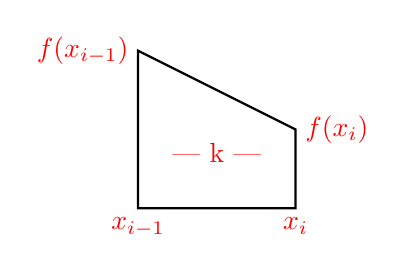
\begin{tikzpicture}
    % Definir los puntos
    \coordinate (A) at (0,2);
    \coordinate (B) at (2,1);
    \coordinate (C) at (2,0);
    \coordinate (D) at (0,0);
    
    % Dibujar el trapecio
    \draw [thick] (A) -- (B) -- (C) -- (D) -- cycle;
    
    % Etiquetas de funciones
    \node[left] at (A) {\textcolor{red}{$f(x_{i-1})$}};
    \node[right] at (B) {\textcolor{red}{$f(x_i)$}};
    \node[below] at (D) {\textcolor{red}{$x_{i-1}$}};
    \node[below] at (C) {\textcolor{red}{$x_i$}};

    % Línea y etiqueta de k dentro del trapecio
    \node[red] at (1,0.7) {\textemdash\ k\ \textemdash};  

\end{tikzpicture}
\caption{Área del trapecio}
\end{figure}

\[
A = \frac{f(x_{i-1}) + f(x_i)}{2} k
\]

\textbf{Solución:}
\[
k = \frac{b-a}{n}
\]

\text{Cuando } n = 20

\[
k = \frac{10}{20} = \frac{1}{2}
\]

\[
t_i = a + k i
\]

\[
t_i = \frac{1}{2} i
\]

\[
f(t_i) = f(x_i) = e^{-\left(\frac{1}{2} i\right)}
\]

\text{Área con trapecios } = A

\[
A = \frac{k}{2} f(x_0) + k \sum_{i=1}^{n-1} f(x_i) + \frac{k}{2} f(x_n)
\]

\[
A = \frac{k}{2} e^{-\left(\frac{1}{2} \cdot 0\right)} + k \sum_{i=1}^{19} e^{-\left(\frac{1}{2} i\right)} + \frac{k}{2} e^{-\left(\frac{1}{2} \cdot 20\right)}
\]

\textbf{Propiedad:} $\quad x^{b \cdot c} = (x^b)^c$

\[
A = \frac{k}{2} \cdot 1 + k \sum_{i=1}^{19} \left( e^{-\frac{1}{2}i} \right) + \frac{k}{2} e^{-10}
\]

\textbf{Propiedad:} 

\[
\sum_{i=0}^{n} x^i = \frac{1 - x^{n+1}}{1 - x}
\]

Si $i = j \Rightarrow$ y $j > 1$

\[
\sum_{i=j}^{n} x^i = \sum_{i=0}^{n} x^i - \sum_{i=0}^{j-1} x^i
\]

\[
\sum_{i=j}^{n} x^i = \frac{1 - x^{n+1}}{1 - x} - \frac{1 - x^j}{1 - x}
\]

\text{Dado que } j-1+1 = j = i, \text{ entonces:}

\begin{equation}
\sum_{i=j}^{n} x^i = \frac{1 - x^{n+1}}{1 - x} - \frac{1 - x^i}{1 - x}
\label{eq:sumatoria}
\end{equation}

\[
\text{Si } \left( e^{\frac{1}{2}} \right) = x \quad \Rightarrow \quad \left( e^{-\frac{1}{2}} \right)^i = x^i
\]

\[
\sum_{i=1}^{19} \left( e^{-\frac{1}{2}} \right)^i = \frac{1 - \left(e^{-\frac{1}{2}}\right)^{20}}{1 - \left(e^{-\frac{1}{2}}\right)} - \frac{1 - \left(e^{-\frac{1}{2}}\right)^{1}}{1 - \left(e^{-\frac{1}{2}}\right)}
\]

\[
\sum_{i=1}^{19} \left( e^{-\frac{1}{2}} \right)^i = \frac{1 - \left(e^{-\frac{1}{2}}\right)^{20}}{1 - \left(e^{-\frac{1}{2}}\right)} - 1
\]

\[
A = \frac{k}{2} \cdot 1 + k \sum_{i=1}^{19} \left( e^{-\frac{1}{2} i} \right) + \frac{k}{2} e^{-10}
\]

\[
A = \frac{k}{2} + k \cdot \frac{1 - \left(e^{-\frac{1}{2}}\right)^{20}}{1 - e^{-\frac{1}{2}}} - 1 + \frac{k}{2} e^{-10}
\]

\[
A = k \left[ \frac{1}{2} + \left( \frac{1 - \left(e^{-\frac{1}{2}}\right)^{20}}{1 - e^{-\frac{1}{2}}} - 1 \right) + \frac{1}{2} e^{-10} \right]
\]

\[
A = \frac{1}{2} \left[ \frac{1}{2} + \left( \frac{1 - \left(e^{-\frac{1}{2}}\right)^{20}}{1 - e^{-\frac{1}{2}}} - 1 \right) + \frac{1}{2} e^{-10} \right]
\]

\[
A = 1.020700699 u^2 \quad \text{para } n = 20
\]

\section{Análisis Numérico usando Python}

\begin{enumerate}
    \item Escriba un código en Python que aproxime \( \int_{0}^{1} e^x dx \) usando el método del trapecio con \( n = 10 \).
\end{enumerate}

\begin{figure}[H]
    \centering
    \includegraphics[scale=0.25]{images/python1.png}
    \label{fig:integralEx}
\end{figure}


\begin{enumerate}
    \setcounter{enumi}{1}
    \item Compare la precisión del método del trapecio y el método de Simpson para \( \int_{0}^{\pi} \sin x dx \).
\end{enumerate}

\begin{figure}[H]
    \centering
    \includegraphics[scale=0.25]{images/python2.png}
    \label{fig:integralSeno}
\end{figure}

Como se ve en la imagen, he escogido un $n$ bastante grande y realmente no hay una diferencia. Usaré un $n = 1$ para ver si hay alguna diferencia.

\begin{figure}[H]
    \centering
    \includegraphics[scale=0.25]{images/python2_1.png}
    \label{fig:integralSeno_Simpson_Trapecio}
\end{figure}

\begin{align*}
    \int_{0}^{\pi} \sin x \,dx 
      &= \left. -\cos x \right|_{0}^{\pi} \\
      &= -\cos \pi - (-\cos 0) \\
      &= -\cos \pi + \cos 0 \\
      &= -(-1) + 1 \\
      &= 2
    \end{align*}

Para \(n = 2\), se han obtenido las siguientes aproximaciones:
\begin{itemize}
    \item \textbf{Método del Trapecio:} \(A_T \approx 1.5708\).
    \item \textbf{Método de Simpson:} \(A_S \approx 2.0947\).
\end{itemize}

El error porcentual se calcula mediante:

\[
\text{Error \%} = \left|\frac{\text{Aproximación} - \text{Valor exacto}}{\text{Valor exacto}}\right| \times 100\%.
\]

\[
\text{Error}_{\text{Trapecio}} = \left|\frac{1.5708 - 2}{2}\right| \times 100\% \approx 21.46\%
\]
\[
\text{Error}_{\text{Simpson}} = \left|\frac{2.0947 - 2}{2}\right| \times 100\% \approx 4.74\%.
\]

El error porcentual para el método de Simpson es significativamente menor que el del método del trapecio, es decir es más preciso.


\begin{enumerate}
    \setcounter{enumi}{2}
    \item Encuentre la integral definida de \( x^3 \) en \([1,2]\).
\end{enumerate}

\begin{figure}[H]
    \centering
    \includegraphics[scale=0.25]{images/python3.png}
    \label{fig:integralCubica}
\end{figure}

\begin{enumerate}
    \setcounter{enumi}{3}
    \item Estime el área bajo la curva \( y = \cos x \) en \([0, \frac{\pi}{2}]\) con el método de Simpson.
\end{enumerate}

\begin{figure}[H]
    \centering
    \includegraphics[scale=0.25]{images/python4.png}
    \label{fig:integralCoseno}
\end{figure}
\section{Ejercicios del libro}

\subsubsection*{Ejercicio 11}

Use la Regla del Punto Medio con el valor dado de \( n \) para aproximar la integral. Redondee cada respuesta a cuatro decimales.


\[
9. \quad \int_{0}^{10} \sin \sqrt{x} \,dx, \quad n = 5
\]

\[
x_i = a + \Delta x \cdot i
\]

\[
x_{i-1} = a + \Delta x (i-1)
\]

\[
x_i^* = \frac{x_i + x_{i-1}}{2}
\]

\[
x_i^* = \frac{a + \Delta x \cdot i + a + \Delta x (i-1)}{2}
\]


\[
x_i^* = \frac{2a + (2i-1) \Delta x}{2}
\]

\[
x_i^* = a + \frac{2i -1}{2} \Delta x
\]

\[
x_i^* = a + \left(i - \frac{1}{2} \right) \Delta x
\]

\[
\Delta x = \frac{10}{5} = 2
\]

\[
x_i^* = \left(i - \frac{1}{2} \right) 2 = 2i -1
\]

\[
f(x_i^*) = \sin \sqrt{2i -1}
\]

\[
A = k \sum_{i=1}^{n} f(x_i^*)
\]

\[
A = 2 \sum_{i=1}^{10} \sin \sqrt{2i -1}
\]


\[
A = 2 \left[ \sin \sqrt{1} + \sin \sqrt{3} + \sin \sqrt{5} + \sin \sqrt{7} + \sin \sqrt{9} \right]
\]

\[
A = 6.4643 \, u^2
\]


\subsubsection*{Ejercicio 13}

Si tiene un sistema algebraico computacional (CAS) que evalúa aproximaciones por punto medio y grafica los rectángulos correspondientes (use los comandos \texttt{middlesum} y \texttt{middlebox} en Maple), verifique la respuesta del Ejercicio 11 e ilustre con un gráfico. Luego, repita con \( n = 20 \) y \( n = 30 \).

Usando MATLAB, se obtienen las siguientes gráficas:

\[
\text{Para } n = 5; \quad f(x) = \sin(\sqrt{x})
\]

\begin{figure}[H]
    \centering
    \includegraphics[scale=0.5]{images/1 n5.jpeg}
    \label{fig:riemann_med}
\end{figure}

\[
\text{Aproximación de la integral (med): } 6.464277
\]


\[
\text{Para } n = 20; \quad f(x) = \sin(\sqrt{x})
\]

\begin{figure}[H]
    \centering
    \includegraphics[scale=0.5]{images/2 n20.jpeg}
    \label{fig:riemann_med_n20}
\end{figure}

\[
\text{Aproximación de la integral (med): } 6.304519
\]


\[
\text{Para } n = 30; \quad f(x) = \sin(\sqrt{x})
\]

\begin{figure}[H]
    \centering
    \includegraphics[scale=0.5]{images/3 n30.jpeg}
    \label{fig:riemann_med_n30}
\end{figure}

\[
\text{Aproximación de la integral (med): } 6.294108
\]

Puede acceder al script de MATLAB en el siguiente enlace: \url{https://github.com/johanP051/tareaII-calculoII/blob/main/latex/analisisComputacional/cas.m}

\subsubsection*{Ejercicio 17}

Expresar el límite como una integral definida en el intervalo dado.


\[
\lim_{n \to \infty} \sum_{i=1}^{n} x_i \sin x_i \Delta x, \quad [0, \pi]
\]

\[
= \int_{0}^{\pi} (x \sin x) \,dx
\]

\textbf{Usando integración por partes:}

\[
\int x \sin x \,dx
\]

\[
\text{Sea } u = x, \quad dv = \sin x \,dx
\]

\[
du = dx, \quad v = -\cos x
\]

Aplicando la fórmula de integración por partes:

\[
\int u dv = uv - \int v du
\]

\[
\int x \sin x \,dx = -x \cos x + \int \cos x \,dx
\]

\[
\int x \sin x \,dx = -x \cos x + \sin x
\]

Evaluamos en los límites de integración:

\[
\int_{0}^{\pi} x \sin x \,dx = \left[ -x \cos x + \sin x \right]_{0}^{\pi}
\]

\[
= \left( -\pi \cos \pi + \sin \pi \right) - \left( -0 \cos 0 + \sin 0 \right)
\]

\[
= (-\pi (-1) + 0) - (0 + 0)
\]

\[
= \pi
\]

\subsubsection*{Ejercicio 19}

\[
\lim_{n \to \infty} \sum_{i=1}^{n} \left[ 2(x_i^*)^2 - 5x_i^* \right] \Delta x, \quad [0,1]
\]

\[
= \int_{0}^{1} (5x^2 - 5x) \,dx
\]

\[
= \int_{0}^{1} 5x(x - 1) \,dx
\]

\subsubsection*{Ejercicio 21}

\[
\int_{-1}^{5} (1 + 3x) \,dx
\]

\[
= \int_{-1}^{5} dx + \int_{-1}^{5} 3x \,dx
\]

\[
= \left[ x \right]_{-1}^{5} + \left[ \frac{3}{2} x^2 \right]_{-1}^{5}
\]

\[
= (5 - (-1)) + \frac{3}{2} \left( 5^2 - (-1)^2 \right)
\]

\[
= 6 + \frac{3}{2} \cdot 24
\]

\[
= 6 + 36
\]

\[
= 42
\]


\subsubsection*{Ejercicio 23}

\[
\int_{0}^{2} (2 - x^2) \,dx
\]

\[
= \left[ 2x - \frac{1}{3}x^3 \right]_{0}^{2}
\]

\[
= 2(2) - \frac{1}{3} (2^3)
\]

\[
= 4 - \frac{8}{3}
\]

\[
= \frac{8}{3}
\]

\subsubsection*{Ejercicio 25}

\[
\int_{1}^{2} x^3 \,dx
\]

\[
= \left[ \frac{1}{4} x^4 \right]_{1}^{2}
\]

\[
= \frac{1}{4} \left[ 2^4 - 1^4 \right]
\]

\[
= \frac{1}{4} \left[ 16 - 1 \right]
\]

\[
= \frac{15}{4}
\]


\subsubsection*{Ejercicio 27}

\[
\int_{0}^{\pi} \sin 5x \,dx
\]

\[
x_i = \frac{\pi}{n} i
\]

\[
\lim_{n \to \infty} \sum_{i=1}^{n} \frac{\pi}{n} \sin \left( \frac{5\pi}{n} i \right)
\]

\textbf{Resolviendo la integral:}

Sabemos que:

\[
\frac{d}{dx} \cos(ax) = -a \sin(ax)
\]

Por lo que:

\[
\int -a \sin(ax) \,dx = a \int -\sin(ax) \,dx
\]

\[
= a \frac{\cos(ax)}{a}
\]

\[
= \cos(ax)
\]

Aplicamos esta propiedad a la integral dada:

\[
\int_{0}^{\pi} \sin(5x) \,dx = \left[ \frac{-\cos(5x)}{5} \right]_{0}^{\pi}
\]

\[
= \frac{-\cos(5\pi)}{5} - \frac{-\cos(0)}{5}
\]

\[
= \frac{-(-1)}{5} - \frac{-1}{5}
\]

\[
= \frac{1 + 1}{5} = \frac{2}{5} = 0.2
\]

\subsubsection*{Ejercicio 29}

\textbf{Se muestra la gráfica de \( f \). Evalúe cada integral interpretándola en términos de áreas.}

\begin{enumerate}[label=(\alph*)]
    \item \( \int_{0}^{2} f(x) \,dx \)
    \item \( \int_{0}^{5} f(x) \,dx \)
    \item \( \int_{5}^{7} f(x) \,dx \)
    \item \( \int_{0}^{9} f(x) \,dx \)
\end{enumerate}

\begin{figure}[H]
    \centering
    \includegraphics[scale=0.3]{images/integral1.png}
\end{figure}

\[
\text{(a)} \quad \int_{0}^{2} f(x)\,dx 
= \frac{3 + 1}{2} \cdot 2 
= 4
\]

\begin{figure}[H]
    \centering
    \includegraphics[scale=0.3]{images/integral2.png}
\end{figure}

\[
\text{(b)} \quad \int_{0}^{5} f(x)\,dx 
= \int_{0}^{2} f(x)\,dx \;+\; \int_{2}^{5} f(x)\,dx 
= 4 \;+\; \frac{3 + 1}{2} \cdot 3 
= 10
\]

\begin{figure}[H]
    \centering
    \includegraphics[scale=0.3]{images/integral3.png}
\end{figure}

\[
\text{(c)} \quad \int_{5}^{7} f(x)\,dx 
= \frac{2(-3)}{2} = -3
\]

\begin{figure}[H]
    \centering
    \includegraphics[scale=0.3]{images/integral4.png}
\end{figure}

\[
\text{(d)} \quad \int_{0}^{9} f(x)\,dx 
= \int_{0}^{5} f(x)\,dx + \int_{5}^{7} f(x)\,dx + \int_{7}^{9} f(x)\,dx
\]

\[
= 10 - 3 - \frac{3+2}{2} \cdot 2
\]

\[
= 10 - 3 - 5
\]

\[
= 2
\]

\begin{figure}[H]
    \centering
    \includegraphics[scale=0.3]{images/integral5.png}
\end{figure}

\subsubsection*{Ejercicio 31}

\[
\quad \int_{1}^{3} (1 + 2x) \,dx
\]

\[
= \int_{1}^{3} 1 \,dx + \int_{1}^{3} 2x \,dx
\]

\[
= \left[ x \right]_{1}^{3} + 2 \left[ \frac{x^2}{2} \right]_{1}^{3}
\]

\[
= (3 - 1) + \left( 3^2 - 1^2 \right)
\]

\[
= 2 + 8
\]

\[
= 10
\]

\section{Ejercicios de clase}

\subsection*{Demostraciones usando diferencias finitas}

\[
\sum_{i=0}^{n} i = \frac{n(n+1)}{2}
\]

Sea \( a_n \) un polinomio, si la \( K \)-ésima diferencia finita de \( a_n \), \( \Delta^K a_n \), es constante, entonces \( a_n \) es un polinomio de grado \( K \).

\begin{itemize}
    \item Primera diferencia finita de \( a_n \):
    \[
    \Delta a_n
    \]
    \item Segunda diferencia finita de \( a_n \):
    \[
    \Delta(\Delta a_n) = \Delta^2 a_n
    \]
    \item Tercera diferencia finita de \( a_n \):
    \[
    \Delta(\Delta^2 a_n) = \Delta^3 a_n
    \]
    \item \( K \)-ésima diferencia finita de \( a_n \):
    \[
    \Delta(\Delta^{K-1} a_n) = \Delta^K a_n
    \]
\end{itemize}

\begin{table}[h]
    \centering
    \begin{tabular}{c|c|c|c|c|c}
        \( n \) & 0 & 1 & 2 & 3 & 4 \\
        \hline
        \( a_n = \sum_{i=0}^{n} i \) & 0 & 1 & 3 & 6 & 10 \\
        \hline
        \( \Delta a_n \) & \(1-0=1\) & \(3-1=2\) & \(6-3=3\) & \(10-6=4\) & \(15-10=5\) \\
        \hline
        \( \Delta^2 a_n \) & \(2-1=1\) & \(3-2=1\) & \(4-3=1\) & \(5-4=1\) &  \\
    \end{tabular}
    \caption{Diferencias finitas de \( a_n \)}
\end{table}

\[
\Delta a_n = a_{n+1} - a_n
\]

\[
\Delta^2 a_n = 1, \quad \forall n \in \mathbb{Z}
\]

Como \( \Delta^2 a_n \) es constante, entonces \( \sum_{j=2}^{n} j \) es un polinomio de grado 2.

\[
a_n = \sum_{i=0}^{n} i = a n^2 + b n + c
\]

Si \( n = 0 \):

\[
a_0 = \sum_{i=0}^{0} i = 0
\]

\[
a_0 = a(0) + b(0) + c = 0
\]

\[
c = 0
\]


Si \( n = 1 \):

\[
a_1 = 1
\]

\[
a_1 = a \cdot 1^2 + b \cdot 1 + 0 = 1
\]

\[
a + b = 1
\]

Si \( n = 2 \):

\[
a_2 = 3
\]

\[
a_2 = a \cdot 2^2 + b \cdot 2 + 0 = 3
\]

\[
4a + 2b = 3
\]

\[
\begin{cases}
a + b = 1 \quad \text{(1)} \\
4a + 2b = 3 \quad \text{(2)}
\end{cases}
\]

De la ecuación (1):

\[
a = 1 - b
\]

De la ecuación (2):

\[
a = \frac{3 - 2b}{4} = \frac{3}{4} - \frac{b}{2}
\]

Igualando ambas expresiones para \( a \):

\[
1 - b = \frac{3}{4} - \frac{b}{2}
\]

\[
1 - \frac{3}{4} = b - \frac{b}{2}
\]

\[
\frac{1}{4} = \frac{b}{2}
\]

\[
b = \frac{1}{2}
\]

\begin{equation*}
    \begin{aligned}
    &\text{Usando la ecuación \textbf{(1)}} \quad a + b = 1 \quad \text{y} \quad b = \frac{1}{2} \\
    &a = 1 - \frac{1}{2} \\
    &a = \frac{1}{2}
    \end{aligned}
\end{equation*}

\[
a_n = a n^2 + b n + c ; \quad a = \frac{1}{2}, \quad b = \frac{1}{2}, \quad c = 0
\]

Cálculo de la sumatoria:

\[
\sum_{i=0}^{n} i = a_n = \frac{1}{2} n^2 + \frac{1}{2} n
\]

Factorizando:

\[
\sum_{i=0}^{n} i = \frac{n^2 + n}{2}
\]

Expresión final:

\[
\sum_{i=0}^{n} i = \frac{n(n+1)}{2}
\]

\section*{Demostración suma de los primeros enteros cuadrados}

\[
\sum_{i=1}^{n} i^2 = \frac{n(n+1)(2n+1)}{6}
\]

\begin{table}[h]
    \centering
    \begin{tabular}{c|c|c|c|c|c}
        \( n \) & 0 & 1 & 2 & 3 & 4 \\ \hline
        \( a_n = \sum_{i=0}^{n} i^2 \) & 0 & 1 & 5 & 14 & 30 \\ \hline
        \( \Delta a_n \) & 1 & 4 & 9 & 16 & 25 \\ \hline
        \( \Delta^2 a_n \) & 3 & 5 & 7 & 9 &  \\ \hline
        \( \Delta^3 a_n \) & 2 & 2 & 2 &  &  
    \end{tabular}
    \caption{Diferencias finitas de la suma de cuadrados}
    \label{tabla_suma_cuadrados}
\end{table}

\[
\Delta^3 a_n = 2 \Rightarrow \Delta^3 a_n \text{ es constante}
\]

\[
a_n = \sum_{i=0}^{n} i^2 = a n^3 + b n^2 + c n + d
\]

\subsection*{Determinación de coeficientes}

\textbf{Caso \( n = 0 \)}

\[
a_0 = \sum_{i=0}^{0} i^2 = 0
\]

\[
a_0 = a \cdot 0^3 + b \cdot 0^2 + c \cdot 0 + d = 0
\]

\[
d = 0
\]

\textbf{Caso \( n = 1 \)}

\[
a_1 = \sum_{i=0}^{1} i^2 = 1
\]

\[
a_1 = a \cdot 1^3 + b \cdot 1^2 + c \cdot 1 + d = 1
\]

\[
a + b + c = 1
\]

\textbf{Caso \( n = 2 \)}

\[
a_2 = \sum_{i=1}^{2} i^2 = 5
\]

\[
a_2 = 8a + 4b + 2c = 5
\]

\textbf{Caso \( n = 3 \)}

\[
a_3 = \sum_{i=1}^{3} i^2 = 14
\]

\[
a_3 = 27a + 9b + 3c = 14
\]

\subsection*{Sistema de ecuaciones}

\[
\begin{cases}
a + b + c = 1 \\
8a + 4b + 2c = 5 \\
27a + 9b + 3c = 14
\end{cases}
\]

\subsection*{Forma matricial}

\[
\begin{pmatrix}
1 & 1 & 1 & | 1 \\
8 & 4 & 2 & | 5 \\
27 & 9 & 3 & | 14
\end{pmatrix}
\]

\[
8F_1 - F_2 \rightarrow F_2
\]

\[
27F_1 - F_3 \rightarrow F_3
\]

\subsection*{Reducción de la matriz}

\[
\frac{1}{18} F_3 - \frac{1}{4} F_2 \rightarrow F_3
\]

\[
\begin{pmatrix}
1 & 1 & 1 & | 1 \\
0 & 4 & 6 & | 3 \\
0 & 18 & 24 & | 13
\end{pmatrix}
\]

\[
\begin{pmatrix}
1 & 1 & 1 & | 1 \\
0 & 4 & 6 & | 3 \\
0 & 0 & -\frac{1}{6} & | -\frac{1}{36}
\end{pmatrix}
\]

\subsection*{Resolviendo el sistema}

\[
a + b + c = 1
\]

\[
4b + 6c = 3
\]

\[
-\frac{1}{6} c = -\frac{1}{36}
\]

\[
c = \frac{1}{6}
\]

\[
b = \frac{3 - 6c}{4}
\]

\[
b = \frac{3 - 1}{4}
\]

\[
b = \frac{2}{4} = \frac{1}{2}
\]

\[
a = 1 - b - c
\]

\[
a = 1 - \frac{1}{2} - \frac{1}{6}
\]

\[
a = \frac{6}{6} - \frac{3}{6} - \frac{1}{6}
\]

\[
a = \frac{1}{3}
\]

\[
a_n = a n^3 + b n^2 + c n
\]

\[
a_n = \frac{1}{3} n^3 + \frac{1}{2} n^2 + \frac{1}{6} n
\]

\[
a_n = \frac{2}{6} n^3 + \frac{3}{6} n^2 + \frac{1}{6} n
\]

\[
a_n = \frac{2n^3 + 3n^2 + n}{6}
\]

\[
a_n = \frac{n(2n^2 + 3n + 1)}{6}
\]

\[
a_n = \frac{n \left( (n+1)(2n+1) \right)}{6}
\]

\[
a_n = \sum_{i=0}^{n} i^2 = \frac{n(n+1)(2n+1)}{6}
\]




\begin{thebibliography}{9}
    \bibitem{1} Stewart J. -- \emph{Calculus Concepts and Contexts}, 2ª ed., Thomson (2004).
    \bibitem{2} Boyce, W. E.; DiPrima, R. C.; Meade, D. B. -- \emph{Elementary Differential Equations and Boundary Value Problems}, Wiley (2021).
    \bibitem{3} Marsden, J.; Tromba, A. -- \emph{Cálculo Vectorial}, (1991).
    \bibitem{4} Apostol, T. -- \emph{Calculus Volumen I: Cálculo con funciones de una variable, con una introducción al álgebra lineal}, 2ª ed., Reverte (2001).
\end{thebibliography}

\end{document}